\documentclass[a4paper,12pt]{extarticle}

% Language setting
% Replace `english' with e.g. `spanish' to change the document language
\usepackage[danish]{babel}

% Set page size and margins
% Replace `letterpaper' with `a4paper' for UK/EU standard size
\usepackage[a4paper,top=2cm,bottom=2cm,left=2cm,right=2cm,marginparwidth=1.75cm]{geometry}


% Useful packages
\usepackage{amsmath}
\usepackage{graphicx}
\usepackage[colorlinks=true, allcolors=black]{hyperref}
\usepackage{tikz}
\usetikzlibrary{calc}
\usepackage{anyfontsize}

\usepackage{minted}

\usepackage[parfill]{parskip}

\usepackage{wrapfig}
\usepackage[utf8]{inputenc}
\usepackage[T1]{fontenc}

% Include images
\graphicspath{ {../img/} }


\begin{document}
    \begin{titlepage}
        \begin{center}
            \vspace{1cm}

            \begin{huge}
                \textbf{RSACrackstation}
            \end{huge}

            \vspace{1cm}

            \textbf{Daniel Nettelfield og Gustav Nybro}

            \vspace{1.5cm}

            \noindent
            
\includegraphics[scale=0.7]{logo}

            \vfill

            En teknologisk og matematisk gennemgang af RSA kryptering\\
            og RSACrackstation projektet, udviklet i forbindelse med\\
            programmeringsfaget på HTX.\@

            \vspace{0.8cm}

            Teknisk Gymnasium Silkeborg\\
            3x\\
            31/10 - 2022

        \end{center}
    \end{titlepage}

    \newpage

    \section*{Abstract}\label{sec:abstract}

    Formålet med projektet er at kunne demonstrere vores tillærte viden fra programmeringsfaget.
    Ved brug af vores ræssonmentskompetence har vi formået at sammesætte et projekt,
    der dækker alle de faglige mål i programmeringsfaget.
    
    Vi har fremstillet en hjemmeside til at behandle RSA, på en brugervenlig og hurtig måde.
    Koden kan tilgåes fra links i bilag og det færdige produkt kan tilgåes på internettet,
    på \href{https://rsacrackstation.com}{rsacrackstation.com}.

    \newpage

    \tableofcontents

    \newpage


    \section{Problemformulering}\label{sec:problemformulering}

    \subsection{Beskrivelse}\label{subsec:beskrivelse}
    Hjemmesiden er en side der kan faktorisere primtal ved hjælp at af API call til en ekstern database.
    Derudover kan hjemmesiden bruges til at bryde krypteringsalgoritmen RSA, og dertil dekryptere indtastet tekst.
    Derudover kan hjemmesiden også bruges til at kryptere tekst med RSA. Hjemmesidens målgruppe er primært CTF
    spillere, cybersikkerheds entusiaster og andre der skal kryptere og dekryptere med RSA\@.

    \subsection{Krav}\label{subsec:krav}
    \begin{itemize}
        \item Hjemmesiden skal kunne faktorisere primtal.
        \item Hjemmesiden skal kunne bryde svag RSA kryptering.
        \item Hjemmesiden skal kunne kryptere med RSA\@.
    \end{itemize}


    \section{Hvad er RSA?}\label{sec:hvad-er-rsa}
    RSA er en asymmetrisk kryptografialgoritme, som er udviklet af Ron Rivest, Adi Shamir og Leonard Adleman i 1977.
    En asymmetrisk kryptografialgoritme er en kryptografialgoritme der bruger to forskellige nøgler til at kryptere og dekryptere,
    og bruges ofte af blandt andet banker, til at sikre deres data.
    Idéen er er man kan offenliggøre krypteringsnøglen, men beholde dekrypteringsnøglen privat, så brugere kan kryptere data på deres egen maskine,
    og sende den krypterede tekst til banken, som dekrypterer den med sin private nøgle.
    RSA nøglerne er genereret ved at bruge to primtal, som er valgt tilfældigt.
    Den offentlige nøgle regnes ved at gange de to primtal sammen, og den private ved at bruge en kompliceret algoritme,
    der hedder den Udvidede Euklidiske Algoritme.\@
    De to tilfældige primtal kaldes \emph{p} og \emph{q}, deres produkt (den offentlige nøgle) kaldes \emph{n}, og den private nøgle kaldes \emph{d}.
    Udover at bruge primtal til at generere RSA nøglerne, bruger RSA også en eksponent, som har en række af krav den skal opfylde,
    alt efter værdierne af de to primtal.
    Dog findes der et tal, som altid kan bruges som eksponent, og det er 65537, denne eksponent kaldes \emph{e}.
    Det sidste tal man bruger i RSA, hedder \emph{m}, og er den værdi man gerne vil sende, ofte en tekst.\@

    \subsection{Hvordan virker RSA?}\label{subsec:hvordan-virker-rsa}
    Når man krypterer med RSA, bruges følgende formel:

    \begin{equation}
        c = m^e \mod n \label{eq:rsa-encrypt}
    \end{equation}

    Her bruges modulus regning, som er måden man sikrer, at den krypterede tekst, ikke kan dekrypteres.
    Modulus virker nemlig ved at tage resten efter en heltalsdivision,
    det vil sige at flere udregninger godt kan give det samme resultat

    \begin{equation}
        2^{11} \mod 527 = 467 \label{eq:encrypt-ex1}
    \end{equation}
    \begin{equation}
        106^{13} \mod 551 = 467 \label{eq:encrypt-ex2}
    \end{equation}

    I dette eksempel, er \(\textbf{m} = 2\), i ligning~\eqref{eq:encrypt-ex1} og \(\textbf{m} = 106\) i ligning~\eqref{eq:encrypt-ex2}.
    Så man kan man se at bare fordi man kender \textbf{c} betyder det ikke at man kender \textbf{m},
    da \textbf{c} er ens i begge eksempler, men \textbf{m} er forskellige.
    For at dekryptere denne tekst skal man bruge værdien for \textbf{d}, som findes ved at faktorisere de to \textbf{n}`er.
    I dette eksempel bruger vi meget små tal, og det er derfor meget nemt at faktorisere de to moduluer.
    Når man har faktoriseret \textbf{n}, kan man køre den udvidede Euklidske algoritme, som bruges til at finde \textbf{d}.
    Hvis man kører denne algoritme på vores to eksempler, får man \(\textbf{d} = 131\) og \(\textbf{d} = 349\).\@
    \textbf{d} kaldes for den inverse af \(\textbf{e} \mod \textbf{n}\), og bruges til at gøre det modsatte af kryptering.
    Når man har regnet \textbf{d}, er det meget enkelt at dekryptere, man skal nemlig gøre det samme som når man kryptere,
    men med \textbf{d} i stedet for \textbf{e}:

    \begin{equation}
        m = c^d \mod n \label{eq:rsa-decrypt}
    \end{equation}

    Hvis man gør dette for vores to eksempler får man dette:

    \begin{equation}
        467^{131} \mod 527 = 2 \label{eq:decrypt-ex1}
    \end{equation}
    \begin{equation}
        467^{349} \mod 551 = 106 \label{eq:decrypt-ex2}
    \end{equation}

    Hvor de to resultater, er de samme to tal, vi krypterede til at starte med, og vi har altså dekrypteret vores tekst.

    \section{Hvad er en API?}\label{sec:hvad-er-en-api}
    API står for Application Programming Interface, hvilket er en måde for noget kode at interagere med noget andet kode.
    En API er modsætningen til en brugergrænseflade, som er en grænseflade rettet mod mennesker.
    API kald kan enten ændre data eller hente data fra en server.
    APIs er overalt på internettet og størstedelen af populære hjemmesider bruger APIs.
    Et godt eksempel på en API der bliver brugt af mange mennesker, er Rejseplanen.
    Rejseplanen fungerer ved at en bruger indtaster noget data, som bliver sendt til backenden.
    Backenden sender kun rå JSON data tilbage, som frontenden behandler og viser på en måde, brugeren lettere kan forestå.


    \section{Frontend}\label{sec:frontend}
    \subsection{Intro}
    For at kunne bruge hjemmesiden ordenligt er det vigtigt med et brugervenligt interface.
    For at kunne lave et brugervenligt interface, skal der bruges HTML, CSS og JavaScript.
    Det er muligt at lave et flot og meget brugervenligt interface med blot normal CSS og JavaScript,
    men for at hurtigere kunne udvikle vores produkt, valgte vi at bruge Tailwind CSS og JQuery i stedet.
    Tailwind CSS er et CSS framework, der han en masse prædefinerede klasser, som kun har én bestemt funktion.
    Man kan derfor hurtigt lave et flot interface, uden at skulle skrive CSS selv, men bare bruge de prædefinerede klasser.
    Tailwind gør det også nemmere at lave et responsivt UI, da hele frameworket er bygget op omkring det.


    \subsection{Tailwind CDN}
    For at kunne bruge Tailwind frameworket, har man flere forskellige muligheder, dog er der to oplagte:
    \begin{enumerate}
        \item Installere Tailwind via NPM
        \item Loade Tailwind med en CDN (Content Delivery Network)
    \end{enumerate}
    Eftersom vi ikke ville gøre det her projekt mere avanceret end nødvendig, og fordi projektet ikke skal hostes i et produktionsmiljø, kan vi godt nøjes med CDN versionen.
    Hvis hjemmesiden skulle bruges i produktion, ville man ikke bruge Tailwind via CDN, fordi det er ressourcer der skal hentes fra en 3. part, hvilket kan give forskellige problemer.
    Hvis Tailwinds servere går ned, går alle hjemmesider der bruger Tailwinds CDN ned, fordi CSS'en ikke kan loades.
    CDN'en indeholder også alle klasser og skal derfor loade mere end nødvendigt, hvilket kan gøre hjemmesiden langsommere.

    \medskip

    Dette projekt var også småt nok, til at det ville tage en betydelig del af tiden, at sætte Tailwind op ordenligt.
    Tailwind via NPM virker kun, hvis der kører en process og scanner HTML-filerne for opdateringer og laver de klasser der mangler.
    Det betyder så også at Tailwind kun indeholder hvad der bliver brugt og intet andet, i modsætning til mange andre CSS frameworks, så som Bootstrap.

    \subsection{Darkmode}
    Alle vores HTML elementer som er blevet ændret med Tailwind, har to forskellige klasser - en til darkmode og en til lightmode.
    Et eksempel kan ses nedenfor

    \begin{minted}[frame=lines,framesep=2mm,baselinestretch=1.2,fontsize=\footnotesize]{html}
        <div class="w-fit dark:text-white text-gray-800">
        ...
    \end{minted}

    I eksemplet ovenfor bliver der oprettet et $<div>$ tag som indeholder nogle elementer.
    Tagget har to klasser der ændrer tekstens farve, som burde overskrive hinanden, men fordi den ene har \emph{dark:} foran,
    bliver den kun brugt når darkmode er slået til.

    \subsection{Hex Auto Toggle}

    Hjemmesiden kan både arbejde med decimaltal og hexadecimaltal, og der er en knap der skifter mellem dem.
    Hvis man kopierer tallet et sted fra, kan man nemt glemme at skifte mellem de to, hvilket vi løser, ved at automatisk 
    skifte mellem dem, afhængig af hvad der er indsat i inputfeltet.
    Koden nedenfor skifter automatisk mellem de to.

    \begin{listing}[!ht]
        \begin{minted}[frame=lines,framesep=2mm,baselinestretch=1.2,fontsize=\footnotesize,linenos]{javascript}
    // Checks if number is pasted and automatically changes state to hex if hex is pasted
    $("#num").bind('paste', function(e) {
        let data = e.originalEvent.clipboardData.getData('text'); // Gets data from clipboard
        if (/[A-Za-z]/g.test(data)) {  // Regex to check if hex is pasted
            if (!isHex){
                updateHexToggle();
            }
        }
        else if (isHex){
            updateHexToggle()
        }
    });
        \end{minted}
        \caption{\protect\href{https://github.com/Zymat-dk/RSACrackstation/blob/main/Views/Home/Index.cshtml}{Views/Home/Index.cshtml, Linje 49 - 60}}
    \end{listing}

    \medskip

    I linje 2 refererer vi til elementet \emph{num}, som er tekstfeltet, hvor man kan indtaste sit tal.
    Efter det tjekker vi om der bliver indsat et tal ind i inputfeltet og laver en funktion,
    som kører hvis der bliver indsat noget.

    \medskip

    I linje 3 initialiserer vi en variabel i local scope, der indeholder dataen i upklipsholderen,
    som læses direkte fra udklipsholderen i stedet for tekstfeltet.
    Dette gør vi fordi værdien af inputfeltet ikke har ændret sig, når funktionen kører.

    \medskip

    I linje 4-8 tjekker vi om dataen fra variablen i linje 3,
    indeholder store eller små bogstaver og kører funktionen \emph{updateHexToggle()} hvis variablen \emph{isHex} er falsk.
    Vi kører funktionen for at opdatere knappen man kan se på hjemmesiden, samt variablen \emph{isHex}.
    If-statementet tjekker om der er bogstaver i teksten, da hexadecimale tal ofte er en blanding mellem bogstaver og tal.
    Dette er ikke en helt sikker måde at skifte mellem tallene, fordi mindre tal nogle gange ikke indeholder bogstaver.
    Det er dog umuligt at tjekke om et tal er hex eller ej, uden at bruge den her metode.
    Eksempelvis kan tallet 33 forstås som både hex og decimal.

    \medskip

    Hvis tallet ikke indeholder bogstaver kører koden mellem linje 9 og 12.
    Denne kode tjekker igen om variablen \emph{isHex} er sand, og kører funktionen \emph{updateHexToggle()}  hvis den er.
    Det tjekker blot om knappen allerede er sat til hex og skifter den tilbage til decimal, hvis teksten der bliver indsat er decimal.

    \subsection{AJAX Call}
    For at frontenden kan kommunikere med backenden, bruger vi et AJAX kald.


    \begin{listing}[!ht]
        \begin{minted}[frame=lines,framesep=2mm,baselinestretch=1.2,fontsize=\footnotesize,linenos]{javascript}
    function factorize() {
        let num = $("#num").val();
        ...
        $.ajax({
            url: "/api/GetFactors",
            type: "POST",
            data: {
                "inputNum": num,
            },
            success: function(data) {
                if (data[0] == -2 || data[1] == -2) { 
                    showSnackbar("FactorDB is currently offline", 0) 
                    $("#p").val("");
                    $("#q").val("");
                    return;
                }
                if (data[0] == -1 || data[1] == -1) { 
                    showSnackbar("Could not factorize", 1) 
                    $("#p").val("");
                    $("#q").val("");
                    return;
                }
                $("#p").val(data[0]);
                $("#q").val(data[1]);
            }
        });
    }
        \end{minted}
        \caption{\protect\href{https://github.com/Zymat-dk/RSACrackstation/blob/main/Views/Home/Index.cshtml}{Views/Home/Index.cshtml, Linje 82 - 127}}
    \end{listing}

    Vi laver en funktion som indeholder AJAX kaldet, for nemmere at kunne sende en forespørgsel til backenden.
    I linje 2, laver vi en variabel, som indeholder dataen fra det første tekstfelt.
    Under linje 2, håndterer vi dataen og tjekker om den overholder forskellige kriterier, men for simplicitet, har vi valgt at undlade denne del her.
    Vi tjekker blot om dataen er noget serveren kan håndtere, og hvis det ikke er, modtager brugeren en fejlbesked.
    Det betyder også at dataen er sikker efter dette punkt og når det skal sendes via AJAX kaldet.

    \medskip

    Fra linje 4 begynder AJAX kaldet.
    Mellem linje 5 og 9 specificerer vi hvilken data, der skal sendes hvorhen og hvordan den skal sendes.
    Dataen sendes til \emph{/api/GetFactors}, som er endpointet for backenden, hvilket betyder at det er stedet backenden og frontende kan kommunikere.
    Den sendes med et POST request, hvilket er en type forespørgsel, man kan sende data med.
    Dataen sendes som et JavaScript objekt, hvilket også er derfor det ikke nødvendigt at sende en `content-type` med.
    Der findes også andre måder at sende dataen med, hvor man ikke bruger et JavaScript objekt, men det her er klart det bedste måde.

    \medskip

    Koden mellem linje 10 - 24, kører hvis funktionen ikke fejler og får en respons fra serveren.
    Dataen der bliver sendt tilbage har formatet [x, y]. Hvor x og y begge er integers.
    Første if-sætning tjekker om dataen er `-2`, hvilket betyder at serveren ikke kunde forbinde til databsen.
    Hvis dette er tilfældes viser den en lille fejlbesked og fjerner en eventuel værdi af $p$ og $q$ felterne, samt returner, hvilket stopper koden fra at køre videre.
    Anden if-sætning tjekker om dataen er `-1`, hvilket betyder at der er sket en generel fejl på serveren.
    Hvis der er sket en generel fejl, viser den igen en lille fejlbesked og tømmer felterne, samt returnerer for at stoppe koden.
    Hvis der ikke er sket nogle fejl, indeholder data-arrayet to tal, som indsættes i felterne $p$ og $q$.


    \section{Backend}\label{sec:backend}
    Backenden er den del af hjemmesiden, som ikke bliver vist til brugeren.
    Det er her vi behandler dataen, som bliver sendt til os fra frontend.
    Vores backend er skrevet i C\#, og bruger objektorienteret programmering, hvor vi laver klasser til at håndtere forskellige ting.

    \subsection{Primtalsfaktorisering}\label{subsec:prime-factorization}
    For at bryde RSA-algoritmen, skal man faktorisere det store tal \textbf{n}, som er produktet af to primtal.
    At faktorisere store tal er en meget svær opgave, som kræver meget tid og mange ressourcer.
    Det er derfor ikke muligt at faktorisere tallet, når brugeren anmoder om det.
    For at løse dette, findes der store databaser af tal, som er faktoriserede.
    Når en bruger indtaster et tal på hjemmesiden, sender vi talet videre til en database, der hedder factordb.
    Factordb er den største database af faktoriserede tal, og den er gratis at bruge.
    Hvis talet findes i databasen, sender vi det tilbage til brugeren, og hvis det ikke findes, sender vi en fejlmeddelelse.
    Vores implementation af dette kan ses nedenfor.
    \begin{listing}[!ht]
        \begin{minted}[frame=lines,framesep=2mm,baselinestretch=1.2,fontsize=\footnotesize,linenos]{csharp}
public string[] GetFactors(){
    string[] factors = { "-1", "-1" };
    var url = $"http://factordb.com/api?query={_n}";
    var request = WebRequest.Create(url);
    request.Method = "GET";
    var data = "";
    ...
    
    dynamic jsonData = JsonObject.Parse(data);
    ...

    for (var i = 0; i < 2; i++){
        factors[i] = jsonData["factors"][i][0].ToString();
    }
    
    return factors;
}
        \end{minted}
        \caption{\protect\href{https://github.com/Zymat-dk/RSACrackstation/blob/main/Backend/RSACracker.cs}{Backend/RSACracker.cs, Linje 42}}
    \end{listing}

    På linje 1 defineres en metode, der hedder \emph{GetFactors()}, som returnere et array af strings.
    Et array er en datastruktur der kan indeholde flere værdier af samme type.
    I dette tilfælde indeholder arrayet to strings, som er de to faktorer der kommer af at faktorisere \textbf{n}.
    På linje 2 initialiseres arrayet med to strings, som er sat til -1.
    \{-1, -1\} er vores default værdi, som vi bruger til at tjekke om vi har fået en faktorisering fra factorDB.\@
    På linje 3 defineres en variabel, der hedder \emph{url}, som er en streng af tekst, der indeholder den url vi skal sende vores API forespørgsel til.
    På linje 4 defineres en variabel, der hedder \emph{request}, som er af typen \emph{WebRequest}.
    WebRequest er en klasse, der indeholder metoder til at sende forespørgsler til en server.
    I dette tilfælde, bruger vi typen af forespørgslen, der hedder `GET`, som er den mest almindelige type af forespørgsler.
    Med en `GET` forespørgsel, kan vi hente data fra en server, uden at ændre noget på den,
    hvilket er det vi ønsker i dette tilfælde.
    På linje 5 definerer vi en ny variabel, af typen string, som hedder \emph{data}.
    Der er her vores respons fra factorDB, skal ligge.
    Derefter kommer der en masse kode, som ikke er vigtig for at forstå hvordan vi bruger API'en.
    På linje 11 definere vi endnu en variabel, der hedder \emph{jsonData}, som er af typen \emph{JsonObject},
    hvilket lader os håndtere JSON data, som vi får fra factorDB.\@
    Derefter kommer der lidt kode, som undersøger om vi får en gyldig respons, dette er ikke nødvendigt at gennegå.
    På linje 12 laver vi en for-løkke, som kører to gange.
    Første gang den kører, sætter vi variablen \emph{i} til 0, og den anden gang sætter vi den til 1.
    Det er her vi henter ændrer værdierne i arrayet, som vi definerede på linje 2.
    Det gør vi ved at læse JSON dataen, og sætte værdierne ind i arrayet til de faktorer vi får fra factorDB.\@
    Til sidst returnerer vi arrayet, som indeholder de faktorer vi har fået fra factorDB.\@

    \newpage

    \subsection{RSA Funktionalitet}\label{subsec:rsa-functionality}
    For at kryptere og dekryptere RSA, skal vi bruge lidt kode.
    Da vi bruger objektorienteret programmering, har vi lavet nogle klasser, en af disse hedder \emph{RSADecrypter},
    som indeholder metoder til at dekryptere.
    Hele klassen kan ses her:
    \begin{listing}[!ht]
        \begin{minted}[frame=lines,framesep=2mm,baselinestretch=1.2,fontsize=\footnotesize,linenos]{csharp}
public class RSADecrypter{
    private BigInteger _n;
    private BigInteger _d;
    private BigInteger _c;
    private BigInteger _m;
    
    public RSADecrypter(string n, string d){
        _n = BigInteger.Parse(n);
        _d = BigInteger.Parse(d);
    }
    
    public string Decrypt(string c){
        _c = BigInteger.Parse(c);
        _m = BigInteger.ModPow(_c, _d, _n);
        return Convert.ToString(_m);
    }
}
        \end{minted}
        \caption{\protect\href{https://github.com/Zymat-dk/RSACrackstation/blob/main/Backend/RSADecrypter.cs}{Backend/RSADecrypter.cs}}
    \end{listing}

    I denne klasse, har vi fire private variable, som er af typen \emph{BigInteger}.
    BigInteger er en klasse, der kan håndtere meget store tal, hvilket vi har brug for, når vi arbejder med RSA.\@
    På linje 7 definerer vi en constructor-metode, som er den metode der kaldes,
    når man initialiserer et objekt af typen \emph{RSADecrypter}.
    Denne metode tager to parametre, som begge er tal, men er af typen string,
    da vi ikke kan håndtere tal af typen BigInteger i frontenden.
    På linje 8 og 9, gemmer vi de to parametre som private variable, som vi kan bruge i andre metoder i klassen.\@
    På linje 12, defineres metoden \emph{Decrypt()}, som tager et tal af typen string, og returnere en string.
    Her tager vi også tal ind som string, for at kunne håndtere det i frontenden.
    På linje 13, gemmer vi det indkommende tal som en private variable, og derefter laver vi en udregning på linje 14.
    Denne udregning blev gennemgået i \autoref{subsec:hvordan-virker-rsa}, og er sådan man dekryptere RSA.\@
    Til sidst returnerer vi resultatet af udregningen som typen string, for at undgå problemer i frontenden.\@

    \section{Test af programmet}\label{sec:testing}

    \subsection{Test af kryptering}\label{subsec:testing-encryption}
    For at teste om vores program virker, har vi lavet en test, som krypterer begge vores navne.
    Vi starter med at generere en nøgle, som vi kan bruge til at kryptere vores navne.
    Derefter indsætter vi nøglen på krypteringssiden, og krypterer vores besked.
    Dette giver et stort tal, som enten kan vises som normalt heltal, eller som et hexadecimalt tal.

    \begin{center}
        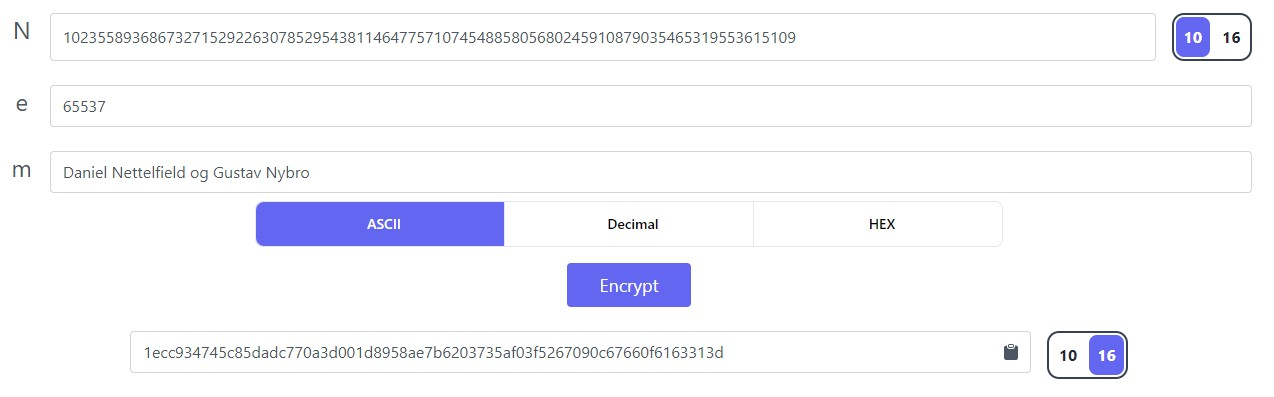
\includegraphics[scale=0.5]{EncryptionLight}\label{img:encryption}
    \end{center}

    \subsection{Test af faktorisering}\label{subsec:testing-factorization}
    For at undersøge om vi kan faktorisere et tal, har vi valgt at lave en svag nøgle,
    så det er muligt at faktorisere den.
    Hvis man indsætter det tal vi brugte til at kryptere, på vores faktoriseringsside, får man følgende resultat:

    \begin{center}
        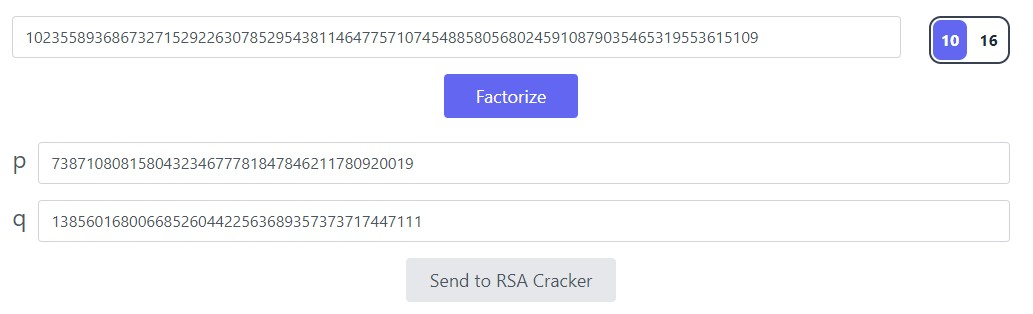
\includegraphics[scale=0.6]{FactorizationLight}\label{img:factorization}
    \end{center}

    Det betyder at vi har fundet de to tal, der kan ganges sammen og give det tal vi startede med.
    Med den information kan man bryde RSA krypteringen, og få beskeden ud.

    \subsection{Test af RSA-brydning}\label{subsec:testing-cracking}
    For at teste om vi kan bryde RSA krypteringen, har vi brugt de to faktorer vi fik fra faktoriseringen,
    sammen med den nøgle vi brugte til at kryptere.
    Hvis man sætter dem ind på vores hjemmeside, sammen med den krypterede tekst, får man dette resultat:

    \begin{center}
        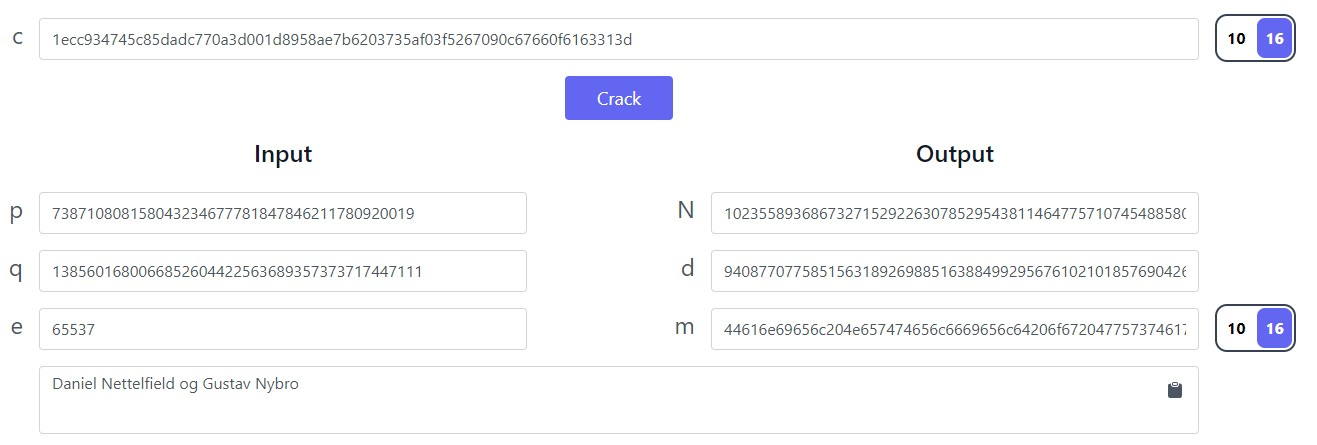
\includegraphics[scale=0.5]{CrackingLight}\label{img:cracking}
    \end{center}

    Her får vi den originale besked ud, hvilket betyder at vi har brudt RSA krypteringen, og bestået alle tests.

    
    \section{Konklusion}\label{sec:konklusion}
    Vi har i dette projekt arbejdet med at bryde RSA kryptering ved hjælp af faktorisering.
    Vi har lavet en hjemmeside, som kan bruges til at kryptere og dekryptere RSA, og til at bryde svag RSA kryptering.
    Vi har været i stand til faktorisere store tal, ved hjælp af kald til en database, 
    som vi kan tilgå ved at bruge en API, udviklet af factorDB, som en den største offentlige faktoriseringsdatabase.
    Udover at kryptere og dekryptere RSA, har vi udviklet en nøglegenerator, som kan generere RSA-nøgler, 
    der er stærke nok til at være sikre mod faktorisering.
    Vi har også lavet en række tests, som viser at vores hjemmeside virker,
    og at vi kan leve op til vores krav om at bryde RSA krypteringen.
    
    \section{Billag}\label{sec:billag}
    \subsection{Kilde Kode - Zip Fil}\label{subsec:billag-source-code}
    \href{https://github.com/Zymat-dk/RSACrackstation/archive/refs/heads/main.zip}{RSACrackstation.zip}
    \subsection{Kilde Kode - Github}\label{subsec:billag-github}
    \href{https://github.com/Zymat-dk/RSACrackstation}{RSACrackstation - Github}
    \subsection{URL - RSACrackstation}\label{subsec:billag-url}
    \href{https://rsacrackstation.com}{rsacrackstation.com}
    
\end{document}
